\documentclass[a4paper]{article}
%\usepackage{utopia}
%\usepackage[adobe-utopia]{mathdesign}
\usepackage{a4wide}
\usepackage{comment}
\usepackage{bcprules}
\usepackage{xspace}
\usepackage{float}
\usepackage{epsfig}
\usepackage{listings}
\usepackage{amsmath}
\usepackage{mathpartir}
\usepackage{wasysym}
\usepackage{stmaryrd}




\def\waebric{\textsc{Waebric}\xspace}
\def\Waebric{\textsc{Waebric}\xspace}
\def\V#1{\ensuremath{\mbox{\textit{#1}}}}
\def\concat{\ensuremath{\;\text{+\hspace{-0.6ex}+}\;}}
\def\hescape#1{\ensuremath{\lfloor #1\rfloor}}
\def\tostring#1{\ensuremath{\llbracket #1 \rrbracket}}

\def\asfsdf{\asf+\-\sdf}
\def\asf{\textsc{Asf}}
\def\sdf{\textsc{Sdf}}

% TODO: use listings
\def\Def{\textbf{def}}
\def\End{\textbf{end}}
\def\If{\textbf{if}}
\def\Each{\textbf{each}}
\def\Else{\textbf{else}}
\def\Yield{\textbf{yield}}
\def\Echo{\textbf{echo}}
\def\Module{\textbf{module}}
\def\Var#1{\textit{#1}}
\def\Site{\textbf{site}}


\floatstyle{boxed}
\newfloat{semantics}{thp}{lop}
\floatname{semantics}{Semantics}


\begin{document}
\title{\waebric: a Little Language for Markup Generation}
\author{Tijs van der Storm}
\date{\today}
\maketitle

\begin{abstract}
  \noindent \waebric\ is a small language for generating XHTML
  markup. Its design is motivated by the lack of programmer friendly
  abstraction facilities in existing markup languages.  \waebric\
  provides a user-friendly syntax to factor Web pages in
  self-contained functional building-blocks. This report introduces
  and motivates \waebric, and presents its syntax and semantics.
\end{abstract}

\section{Introduction}

\subsection{Motivation}

\begin{itemize}
\item (X)HTML is too verbose to be typed (or read) by humans.
\item Template languages feature elaborate quoting schemes that make
  designing templates form (X)HTML even more cumbersome.
\item Template languages often do not allow functional abstraction
  and/or recursion.
\item Template languages do not support ``around'' parameterization
  where one can reuse a piece of markup with one or more holes in it.
\item Template languages often allow arbitrary computation thus
  violating separation of concerns guidelines.
\item WYSIWYG editors have their own issues like generating
  inaccessible and unmaintainable XHTML code.
\end{itemize}



\subsection{What \waebric offers}

\section{A Taste of  \waebric}

The basic \Waebric\ program consists of a number function definitions,
possibly partitioned over a number of modules, together with a site
definition which maps \Waebric\ markup expressions to XHTML files. A
simple \Waebric\ example is displayed below:
\begin{quote}
\begin{tabbing}
\Def\=\ main\\
\>layout("Hello") \{ h1 "Hello World!"; p "Home"; \}\\
\End\\
\Def\=\ layout(\Var{title})\\
\>htm\=l \{ head title \Var{title}; body \Yield; \}\\
\End
\end{tabbing}
\end{quote}


Running this program produces a single XHTML document which consists of
the markup generated by the function main. The main function calls
another function, called layout, which receives an string argument
``Hello''. Additionally, a block (enclosed in curly braces) is passed
to layout. This block will be evaluated wherever the statement
\textbf{yield} occurs within the implementation body of layout. The
block itself consists of two ``function calls'', to h1 and p. Since no
definition exists for h1, this will produce a XHTML ``h1'' element with
the string ``Hello World!'' as content. Subsequently a paragraph is
rendered containing the string ``Home''.

The layout function defines a skeleton page framework that can be
reused across different pages. In the example it sets up a basic XHTML
document with header and title; the body of a page is obtained from
the block passed into it. Note how nesting of elements along a single
spine in the document tree requires no curly braces (as can be seen
from how the title element is included in the head element).

Running this example will produce the following (XHTML) markup:
\begin{quote}\small
$<$html$>$
 $<$head$>$$<$title$>$Hello$<$/title$>$$<$/head$>$
 $<$body$>$
  $<$h1$>$\\Hello World!$<$/h1$>$
  $<$p$>$Home$<$/p$>$
 $<$/body$>$
$<$/html$>$
\end{quote}

In addition to the basic markup generating function calls, as
illustrated by the example, \Waebric\ contains an if-then-else
statement, an each statement, for iterating over sequences of values,
a let construct for the introduction of local variables and local
redefinition of functions and string interpolation syntax (for
embedding markup directly in text).

\begin{figure}
\begin{minipage}{0.6\linewidth}
\begin{tabbing}
\Def\=\ menu(\Var{menu})\\
\>\Echo\ \Var{menu}.title;\\
\>ul\=\ \{\\
\>\>\Each\=\ (kid: menu.kids)\\
\>\>\>menu-item(kid); \\
\>\}\\
\End\\
\\
\Def\ menu-item(\Var{item})\\
\>\If\=\ (\Var{item}.kids) \\
\>\>li menu(\Var{item});\\
\>\Else\\
\>\>li a(\Var{href}=\Var{item}.link) \Var{item}.title;\\
\End
\end{tabbing}
\end{minipage}
\begin{minipage}[b]{0.4\linewidth}
\begin{center}
\fbox{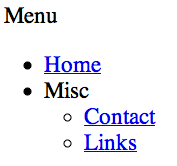
\epsfig{file=Generated-Menu,width=0.5\linewidth}}
\end{center}
\end{minipage}
\caption{Recursive menus in \Waebric\ and the possible
  output\label{FIG:menus}}
\end{figure}

The example in Figure~\ref{FIG:menus} shows how recursive menus could
be defined in \Waebric. The first function, menu, receives a data
object (\Var{menu}) containing the labels, URLs and sub-menus that
should be rendered in XHTML. The next statement just renders the title
of the (current) menu using the built in statement echo. After
the title follows an unordered list containing the items of this
menu. For each element in the ``kids'' property of \Var{menu} the
menu-item function is called.

The menu-item function first checks whether this \Var{item} has any
children (sub-menus). If so, it produces a li(st) element containing
the output of a recursive call to menu. If there are no sub-menus,
the result is a list element with an anchor tag which links the title
of item to its URL. The result of an invocation (with the appropriate
data for the \textit{menu} parameter) of menu could look like the
screen shot next to the source code.

\section{Syntax}



\subsection{Corner cases}

\begin{itemize}
\item An identifier interpolated in a string is parsed as an
  expression whereas an identifier as a statement is parsed as markup
  (e.g. a function call or an XHTML element construction).
\item An identifier in that last position of a markup chain/spine is
  parsed as an expression (not as markup). 
\end{itemize}

\section{Semantics}


\subsection{Abstract Syntax}

See Figure~\ref{FIG:abstract-syntax}.

\begin{figure}
\begin{minipage}[t]{0.33\linewidth}
\[
\begin{array}{rcl}
S & ::= & \text{\textbf{echo} }E \\
& | & \text{\textbf{comment} }E \\
& | & \text{\textbf{cdata} }E\\
& | & \text{\textbf{yield}}\\
& | & \text{\textbf{if} }(P)\;S \text{ \textbf{else} }S\\
& | & \text{\textbf{if} }(P)\;S \\
& | & \text{\textbf{each} }(X: E)\;S\\
& | & \text{\textbf{let} }B\text{ \textbf{in} }S\text{ \textbf{end}}\\
& | & S; S\\
& | & M\; S\\
& | & M\; E\\
& | & M
\end{array}
\]
\end{minipage}
\begin{minipage}[t]{0.33\linewidth}
\[
\begin{array}{rcl}
M & ::= & M\;M\\
& | & f\\
& | & f(A)\\
A & ::= & E\\
& | &X = E\\
& | & A, A\\
E & ::= & X \\
& | & I \\
& | & [\overline{E}]\\
& | & \{ \overline{X : E}\}\\
I & ::= & \V{String} \langle M\; E \rangle I\\
  & | & \V{String} \langle E \rangle I\\
  & | & \V{String}
\end{array}
\]
\end{minipage}
\begin{minipage}[t]{0.33\linewidth}
\[
\begin{array}{rcl}
B & ::= & X = E \\
& | & f(\overline{X}) = S\\
& | & B ; B\\
P & ::= & E\\
& | & E.\text{record?}\\
& | & E.\text{list?}\\
& | & !P \\
& | & P\; \&\&\; P\\
& | & P\; ||\; P\\
\end{array}
\]
\end{minipage}
\caption{Abstract syntax of \waebric\label{FIG:abstract-syntax}}
\end{figure}

\subsection{Semantics}

Figure~\ref{FIG:semantics} shows a natural semantics of \waebric.

\subsubsection{Escaping}
\waebric programs produce XHTML.  The following rules with respect to
escaping should be observed:
\begin{itemize}
\item Any string literal occurring in a \waebric program should
  observe XML escaping rules; this is enforced by the \waebric
  parser. 
\item Data coming from the outside (the model) should be properly
  escaped upon interpolation. An interpreter for \waebric should
  detect data from the outside (tainted data) and apply the proper
  escaping. The locations where an interpreter \textit{must} check if
  a value is tainted or not (and perform escaping if so) are indicated
  with the \hescape{} function.
\item For comments and CDATA sections special escaping rules apply
  (TODO: to be determined).
\end{itemize}

\begin{comment}
\[
\begin{array}{rcl}
\text{\textbf{if}} (p)\; S &\equiv& \text{\textbf{if} } (p)\; S \text{ \textbf{else} \textbf{echo} } \text{``''}\\
\end{array}
\]
\end{comment}


\begin{semantics}\footnotesize
\begin{mathpar}
\inferrule*[right=Var]{
\Gamma(x) = v
}{
\Gamma, \Lambda \vdash_E x \rightarrow v
}

\inferrule*[right=Literal]{ 
}{
\Gamma, \Lambda \vdash_E L \rightarrow L
}

\inferrule*[right=Lookup]{ 
\Gamma, \Lambda \vdash_E e \rightarrow v\\
v \in \text{\textsf{Record}}\\
 (x : v) \in v
}{
\Gamma, \Lambda \vdash_E e.x \rightarrow v
}

\inferrule*[right=Interpolate-1]{
\Gamma \vdash_{E} \V{e} \rightarrow v\\
\Gamma, \Lambda \vdash_E \V{I} \rightarrow s_2
}{
\Gamma, \Lambda \vdash_E s_1 \langle e \rangle \V{I} \rightarrow
s_1 \concat \hescape{v} \concat s_2
}

\inferrule*[right=Interpolate-2]{
\Gamma \vdash_{E} \V{e} \rightarrow v\\
\Gamma, \Lambda, \hescape{v} \vdash_M \V{M} \rightarrow s_2\\
\Gamma, \Lambda \vdash_E \V{I} \rightarrow s_3
}{
\Gamma, \Lambda \vdash_E s_1 \langle M\; e \rangle \V{I} \rightarrow
s_1 \concat s_2 \concat s_3
}

\inferrule*[right=Defined]{
\Gamma, \Lambda \vdash_E e \rightarrow v
}{
\Gamma, \Lambda \vdash_P e
}

\inferrule*[right=IsList]{
\Gamma, \Lambda \vdash_E e \rightarrow v\\
v\in \text{\textsf{List}}
}{
\Gamma, \Lambda \vdash_P e.\text{list?}
}

\inferrule*[right=IsRecord]{
\Gamma, \Lambda \vdash_E e \rightarrow v\\
v \in \text{\textsf{Record}}
}{
\Gamma, \Lambda \vdash_P e.\text{record?}
}

\inferrule*[right=Or-1]{
\Gamma, \Lambda \vdash_P p_1
}{
\Gamma, \Lambda \vdash_P p_1\;||\;p_2
}

\inferrule*[right=Or-2]{
\Gamma, \Lambda \vdash_P p_2
}{
\Gamma, \Lambda \vdash_P p_1\;||\;p_2
}

\inferrule*[right=And]{
\Gamma, \Lambda \vdash_P p_1\\
\Gamma, \Lambda \vdash_P p_2
}{
\Gamma, \Lambda \vdash_P p_1\;\&\&\;p_2
}

\inferrule*[right=Not]{
\Gamma \not\vdash_P p
}{
\Gamma, \Lambda \vdash_P \;!p
}

%\end{mathpar}
%\caption{Semantics of expressions and predicates\label{SEM:expressions}}
%\end{semantics}


%\begin{semantics}\footnotesize
%\begin{mathpar}
\inferrule*[right=echo]{
\Gamma, \Lambda \vdash_E e \rightarrow v
}{
\Gamma, \Lambda, \beta \vdash_S \text{\textbf{echo} }e \rightarrow \hescape{v}
}


\inferrule*[right=Yield]{ 
}{
\Gamma, \Lambda, \beta \vdash_S \text{\textbf{yield}} \rightarrow \beta
}


\inferrule*[right=Comment]{
\Gamma, \Lambda \vdash_E e \rightarrow v
}{
\Gamma, \Lambda, \beta \vdash_S \text{\textbf{comment} }e \rightarrow
\text{``$<$!$-$$-$''} \concat \tostring{v}\backslash\text{``$-$$-$$>$''} \concat \text{``$-$$-$$>$''}
}

\inferrule*[right=CData]{
\Gamma, \Lambda \vdash_E e \rightarrow v
}{
\Gamma, \Lambda, \beta \vdash_S \text{\textbf{cdata} }e \rightarrow
\text{``$<$![CDATA[''} \concat \tostring{v}\backslash\text{``]]$>$''} \concat \text{``]]$>$''}
}

\inferrule*[right=If-1]{
\Gamma, \Lambda \vdash_P p\\
\Gamma, \Lambda, \beta \vdash_S S_1 \rightarrow s_1
}{
\Gamma, \Lambda, \beta \vdash_S \text{\textbf{if} }(p)\; S_1 \text{
  \textbf{else} } S_2 \rightarrow s_1
}

\inferrule*[right=If-2]{
\Gamma, \Lambda \vdash_P\; !p\\
\Gamma, \Lambda, \beta \vdash_S S_2 \rightarrow s_2
}{
\Gamma, \Lambda, \beta \vdash_S \text{\textbf{if} }(p)\; S_1 \text{
  \textbf{else} }S_2 \rightarrow s_2
}

\inferrule*[right=Sequence]{
\Gamma, \Lambda, \beta \vdash_S S_1 \rightarrow s_1\\
\Gamma, \Lambda, \beta \vdash_S S_2 \rightarrow s_2\\
}{
\Gamma, \Lambda, \beta \vdash_S S_1;\; S_2 \rightarrow s_1\concat s_2
}


\inferrule*[right=Each]{
\Gamma, \Lambda \vdash_E e \rightarrow [v_1, ..., v_n]\\
1 \leq i \leq n\\
\Gamma[x/v_i], \Lambda, \beta \vdash_S S \rightarrow s_i\\
}
{
\Gamma, \Lambda, \beta \vdash_S \text{\textbf{each} }(x: e)\; S 
\rightarrow \sum^n_{i = 1} s_i
}

\inferrule*[right=Let]{
\Gamma, \Lambda \vdash_B B \rightarrow \langle\Gamma', \Lambda'\rangle\\
\Gamma', \Lambda', \beta \vdash_S S \rightarrow s
}{
\Gamma, \Lambda, \beta \vdash_S \text{\textbf{let} } B
\text{ \textbf{in} } S \text{ \textbf{end}}\rightarrow s
}

\inferrule*[right=Markup-1]{
\Gamma, \Lambda, \beta \vdash_S S \rightarrow \beta'\\
\Gamma, \Lambda, \beta' \vdash_M M \rightarrow s'
}{
\Gamma, \Lambda, \beta \vdash_S M \; S \rightarrow s'
}


\inferrule*[right=Markup-2]{
\Gamma, \Lambda  \vdash_E e \rightarrow v\\
\Gamma, \Lambda, \hescape{v} \vdash_M M \rightarrow s'
}{
\Gamma, \Lambda, \beta \vdash_S M \; e \rightarrow s'
}

\inferrule*[right=Markup-3]{
\Gamma, \Lambda, \beta \vdash_M M \rightarrow s
}{
\Gamma, \Lambda, \beta \vdash_S M \rightarrow s
}



\inferrule*[right=Bindings]{
\Gamma, \Lambda \vdash_B B_1 \rightarrow\langle \Gamma_1, \Lambda_1\rangle\\
\Gamma_1, \Lambda_1 \vdash_B B_2 \rightarrow\langle \Gamma_2, \Lambda_2\rangle
}{
\Gamma, \Lambda \vdash_B B_1; B_2 \rightarrow \langle \Gamma_2, \Lambda_2\rangle
}

\inferrule*[right=Bindings-Var]{
\Gamma, \Lambda \vdash_E e \rightarrow v
}{
\Gamma, \Lambda \vdash_B x = e \rightarrow \langle\Gamma[x/v], \Lambda\rangle
}

\inferrule*[right=Bindings-Func]{
C = \langle\Gamma, \Lambda, \lambda x_1, ..., x_n\;S\rangle\\
}{
\Gamma, \Lambda \vdash_B f(x_1, ..., x_n) = S \rightarrow 
\langle\Gamma, \Lambda[f/C]\rangle
}

\inferrule*[right=Nest]{
\Gamma, \Lambda, \beta \vdash_M M_2 \rightarrow \beta'\\
\Gamma, \Lambda, \beta' \vdash_M M_1 \rightarrow s 
}
{\Gamma, \Lambda, \beta \vdash_M M_1\; M_2 \rightarrow s}


\inferrule*[right=Empty]{
f \not\in \text{dom}(\Lambda)\\
}{
\Gamma, \Lambda, \beta \vdash_M f \rightarrow
\text{``$<$''} \concat \tostring{\V{f}}\; \concat \text{``/$>$''}
}


\inferrule*[right=Element]{
f \not\in \text{dom}(\Lambda)\\
1 \leq i \leq n+1\\
\Gamma, \Lambda \vdash_E e_i\rightarrow v_i\\
s =\sum^{n+1}_{i = 1} \text{``\textvisiblespace''} \concat \tostring{x_i}
\concat \text{``$\backslash$"''} \concat \hescape{v_i} \concat \text{``$\backslash$"''}
}
{
\Gamma, \Lambda, \beta \vdash_M f(x_1 = e_1, ..., x_{n+1} = e_{n+1}) \rightarrow
\text{``$<$''} \concat \tostring{\V{f}}\; \concat s \concat \text{``$>$''}\concat \beta\concat
\text{``$<$/''} \concat \tostring{\V{f}} \concat \text{``$>$''}
}

\inferrule*[right=Call]{
\Lambda(f) = \langle \Gamma', \Lambda', \lambda x_1,...,x_n\; S\rangle\\
1 \leq i \leq n \\
\Gamma, \Lambda \vdash_E e_i \rightarrow v_i\\
\Gamma[x_1/v_1]...[x_n/v_n],\Lambda, \beta \vdash_S S \rightarrow s
}{
\Gamma, \Lambda, \beta \vdash_M f(e_1,...,e_n) \rightarrow  s
}


\end{mathpar}
\caption{Semantics of statements and markup forms\label{FIG:semantics}}
\end{semantics}



\end{document}


\inferrule*[right=Call0]{
\Lambda(f) = \langle \Gamma', \Lambda',  S\rangle\\
\Gamma', \Lambda', \beta \vdash_S S \rightarrow  s
}{
\Gamma, \Lambda, \beta \vdash_M f \rightarrow  s
}


\inferrule*[right=Implicit-1]{}{
\vdash_I t.x \rightarrow [\text{class}/x]
}

\inferrule*[right=Implicit-2]{}{
\vdash_I t\#x \rightarrow [\text{id}/x]
}

\inferrule*[right=Implicit-3]{}{
\vdash_I t\$x \rightarrow [\text{name}/x]
}


\inferrule*[right=Implicit-4]{}{
\vdash_I t: x \rightarrow [\text{type}/x]
}

\inferrule*[right=Implicit-5]{}{
\vdash_I t @ x \% y \rightarrow [\text{width}/x][\text{height}/y]
}


\inferrule*[right=If-3]{
\Gamma, \Lambda, \beta \vdash_S \text{\textbf{if} }(p)\; S \text{
  \textbf{else} \textbf{echo} ``''} \rightarrow s
}{
\Gamma, \Lambda, \beta \vdash_S \text{\textbf{if} }(p)\; S \rightarrow s
}


\inferrule*[right=Bindings]{
n = |\overline{B}|\\
1 \leq i \leq n\\
\sum_{0 \leq j < i} \Gamma_j,
\sum_{0 \leq j < i} \Lambda_j,
 \vdash_B \langle \Gamma_i, \Lambda_i\rangle\\
}{
\Gamma_0, \Lambda_0 \vdash_B \overline{B} \rightarrow \langle \Gamma_n, \Lambda_n\rangle
}



\inferrule*[right=Call0]{
\Lambda(f) = \langle \Gamma', \Lambda',  S\rangle\\
\Gamma,\Lambda, \beta \vdash_S S \rightarrow s
}{
\Gamma, \Lambda, \beta \vdash_M f \rightarrow s
}
